%------------------------
% DOCUMENT CONFIGURATIONS
%------------------------

% 10pt font size, A4 paper, two-sided margins, book style
\usepackage[top=3.5cm,bottom=3.5cm,left=2cm,right=2cm,columnsep=30pt]{geometry} % Set document margins and spacing

% Custom colors
\usepackage[svgnames]{xcolor}
% word color is an aqua blue
\definecolor{wordColor}{RGB}{29,119,168}
\definecolor{headerLineColor}{RGB}{210,225,230}
% cover page background color is red
% also, this is used as the color for the translucent background to highlight the titles on the cover
\definecolor{backgroundColor}{rgb}{0.68, 0.05, 0.0}
% colored bar at the top of chapters is pale red
\definecolor{headerbackgroundColor}{rgb}{0.9, 0.56, 0.67}
% chapter title backround color is darker red
\definecolor{headertitleColor}{rgb}{0.68, 0.05, 0.0}
% chapter title text is white
\definecolor{headertitletextColor}{RGB}{255, 255, 255}
% titles on the cover are white
\definecolor{covertextColor}{rgb}{1.0, 1.0, 1.0}
% But titles on the title page are black
\definecolor{titletextColor}{RGB}{0, 0, 0}
% title page background color is pale red
\definecolor{titlebackgroundColor}{rgb}{0.9, 0.56, 0.67}
% Some other colors for quick reference
% an easy RGB color picker is at https://www.rapidtables.com/web/color/RGB_Color.html
% blue {RGB}{0,0,204}
% pale blue {RGB}{153, 153, 255}
% dark green {RGB}{0, 153,0}
% pale green {RGB}{102,255,102}
% dark purple {RGB}{76,0,153}
% light purple {RGB}{178,102,255}
% Very Peri - 2022 Pantone color of the year {RGB}{104,104,171}
% dark orange {RGB}{204,102,0}
% light orange {RGB}{255,204,1530}

% Custom fonts
\usepackage[utf8]{inputenc} % For unicode characters
\usepackage[T1]{fontenc} % For unicode characters
\usepackage{fontspec} % For imported font files
\setmainfont{NotoSans-Regular.ttf} % Main font
\newfontfamily{\conWord}[Color=wordColor]{NotoSans-Bold.ttf} % Font style for conlang word (cw)
\newfontfamily{\engWord}[Color=wordColor]{NotoSans-Bold.ttf} % Font style for English word (ew)
\newfontfamily{\engTrans}{CharisSILR.ttf} % Font style for English translation (et)
\newfontfamily{\conTrans}{CharisSILR.ttf} % Font style for conlang translation (ct)
\newfontfamily{\ipa}{CharisSILR.ttf} % IPA pronunciation font
\newfontfamily{\italic}{CharisSILI.ttf} % Part of Speech font
\newfontfamily{\bold}{NotoSans-Bold.ttf} % Black bold Noto

% Fancy header and footer
\usepackage{fancyhdr}
\fancyhead[L]{\textnormal{\color{wordColor}\rightmark}} % Top left header
\fancyhead[R]{\textnormal{\color{wordColor}\leftmark}} % Top right header
\renewcommand{\headrulewidth}{2.4pt} % Width of line under the header
\renewcommand{\headrule}{\hbox to\headwidth{\color{headerLineColor}\leaders\hrule height \headrulewidth\hfill}} % Color of header line
\renewcommand{\footrulewidth}{0pt} % Set footer line to 0pt
\renewcommand{\footrule}{\hbox to\headwidth{\color{headerLineColor}\leaders\hrule height \footrulewidth\hfill}} % Color of footer line
\fancyfoot[C]{{\textsf{\color{wordColor}\thepage}}} % Page number (\thepage), color and centered with [C]
\pagestyle{fancy} % Use the custom headers and footers throughout the document

% Remove automatic paragraph indenting
\usepackage{changepage}
\setlength{\parindent}{0cm}
\newcommand{\forceindent}{\leavevmode{\parindent=0.5em\indent}} % Use custom command \forceindent to indent text

% Conlang entry (ce) and English entry (ee) commands have [3] sections: #1 is the bold word, #2 is the IPA pronunciation, #3 is the translation information. markboth{}{} prints the first word on the page in the top left header and the last word in the top right. {adjustwidth} indents the translation under the word and IPA by 0.2cm
\newcommand{\con}[3]{\conWord{#1}\markboth{#1}{#1}\ \ipa{#2}\engTrans{#3}}
\newcommand{\eng}[3]{\engWord{#1}\markboth{#1}{#1}\ \ipa{#2}\conTrans{#3}}
\newcommand{\pos}[2]{\begin{adjustwidth}{0.2cm}{}{\italic#1} {#2}\end{adjustwidth}}

% Heading styling
\usepackage[explicit]{titlesec}
\usepackage{tikz}

% Chapter styling
\newcommand*\chapterlabel{}
\titleformat{\chapter}
  {\gdef\chapterlabel{}
   \normalfont\sffamily\Huge\bfseries\scshape}
  {\gdef\chapterlabel{}}{0pt}
  {\begin{tikzpicture}[remember picture,overlay]
    \node[yshift=-3cm] at (current page.north west)
      {\begin{tikzpicture}[remember picture, overlay]
        \draw[fill=headerbackgroundColor] (0,0) rectangle
          (\paperwidth,3cm);
        \node[anchor=east,xshift=.9\paperwidth,rectangle,
              rounded corners=20pt,inner sep=11pt,
              fill=headertitleColor]
              {\color{headertitletextColor}\chapterlabel#1};
       \end{tikzpicture}
      };
   \end{tikzpicture}
  }
\titlespacing*{\chapter}{0pt}{10pt}{-20pt}
  
% Section styling
\newcommand*\sectionlabel{}
\titleformat{name=\section,numberless}
  {\normalfont\Huge\bfseries\filcenter}
  {\thesectionlabel#1}
  {1em}
  {}
  [{\titlerule[0.8pt]}]

% Subsection styling

\titleformat{name=\subsection,numberless}
  {\b\Large}
  {}
  {.5em}
  {}
% Other misc. packages
\usepackage{multicol} % For multiple columns
\usepackage{caption} % For table captions
\usepackage{microtype} % Improves spacing
\usepackage{needspace} % For page breaking
\usepackage{titling}

% Publisher logo
\usepackage{graphicx}
\usepackage{marvosym}
\newcommand*{\titlelogo}{Vulgarlang.com~~\fbox{$\mathcal{VL}$}}
% cover logo - the world icon is from the marvosym wingdings font
\newcommand*{\coverlogo}{A Many Worlds Project~~\Huge{\Mundus}}

%Stops dictionary entries breaking over columns
\makeatletter
\newcommand*\nobreaklist{\@beginparpenalty=\@M}
\makeatother
\nobreaklist

% commands for adding a picture to the cover
\usepackage{eso-pic}
% this is the full page cover picture
\newcommand\BackgroundPicFull{
\AddToShipoutPicture{\put(0,0){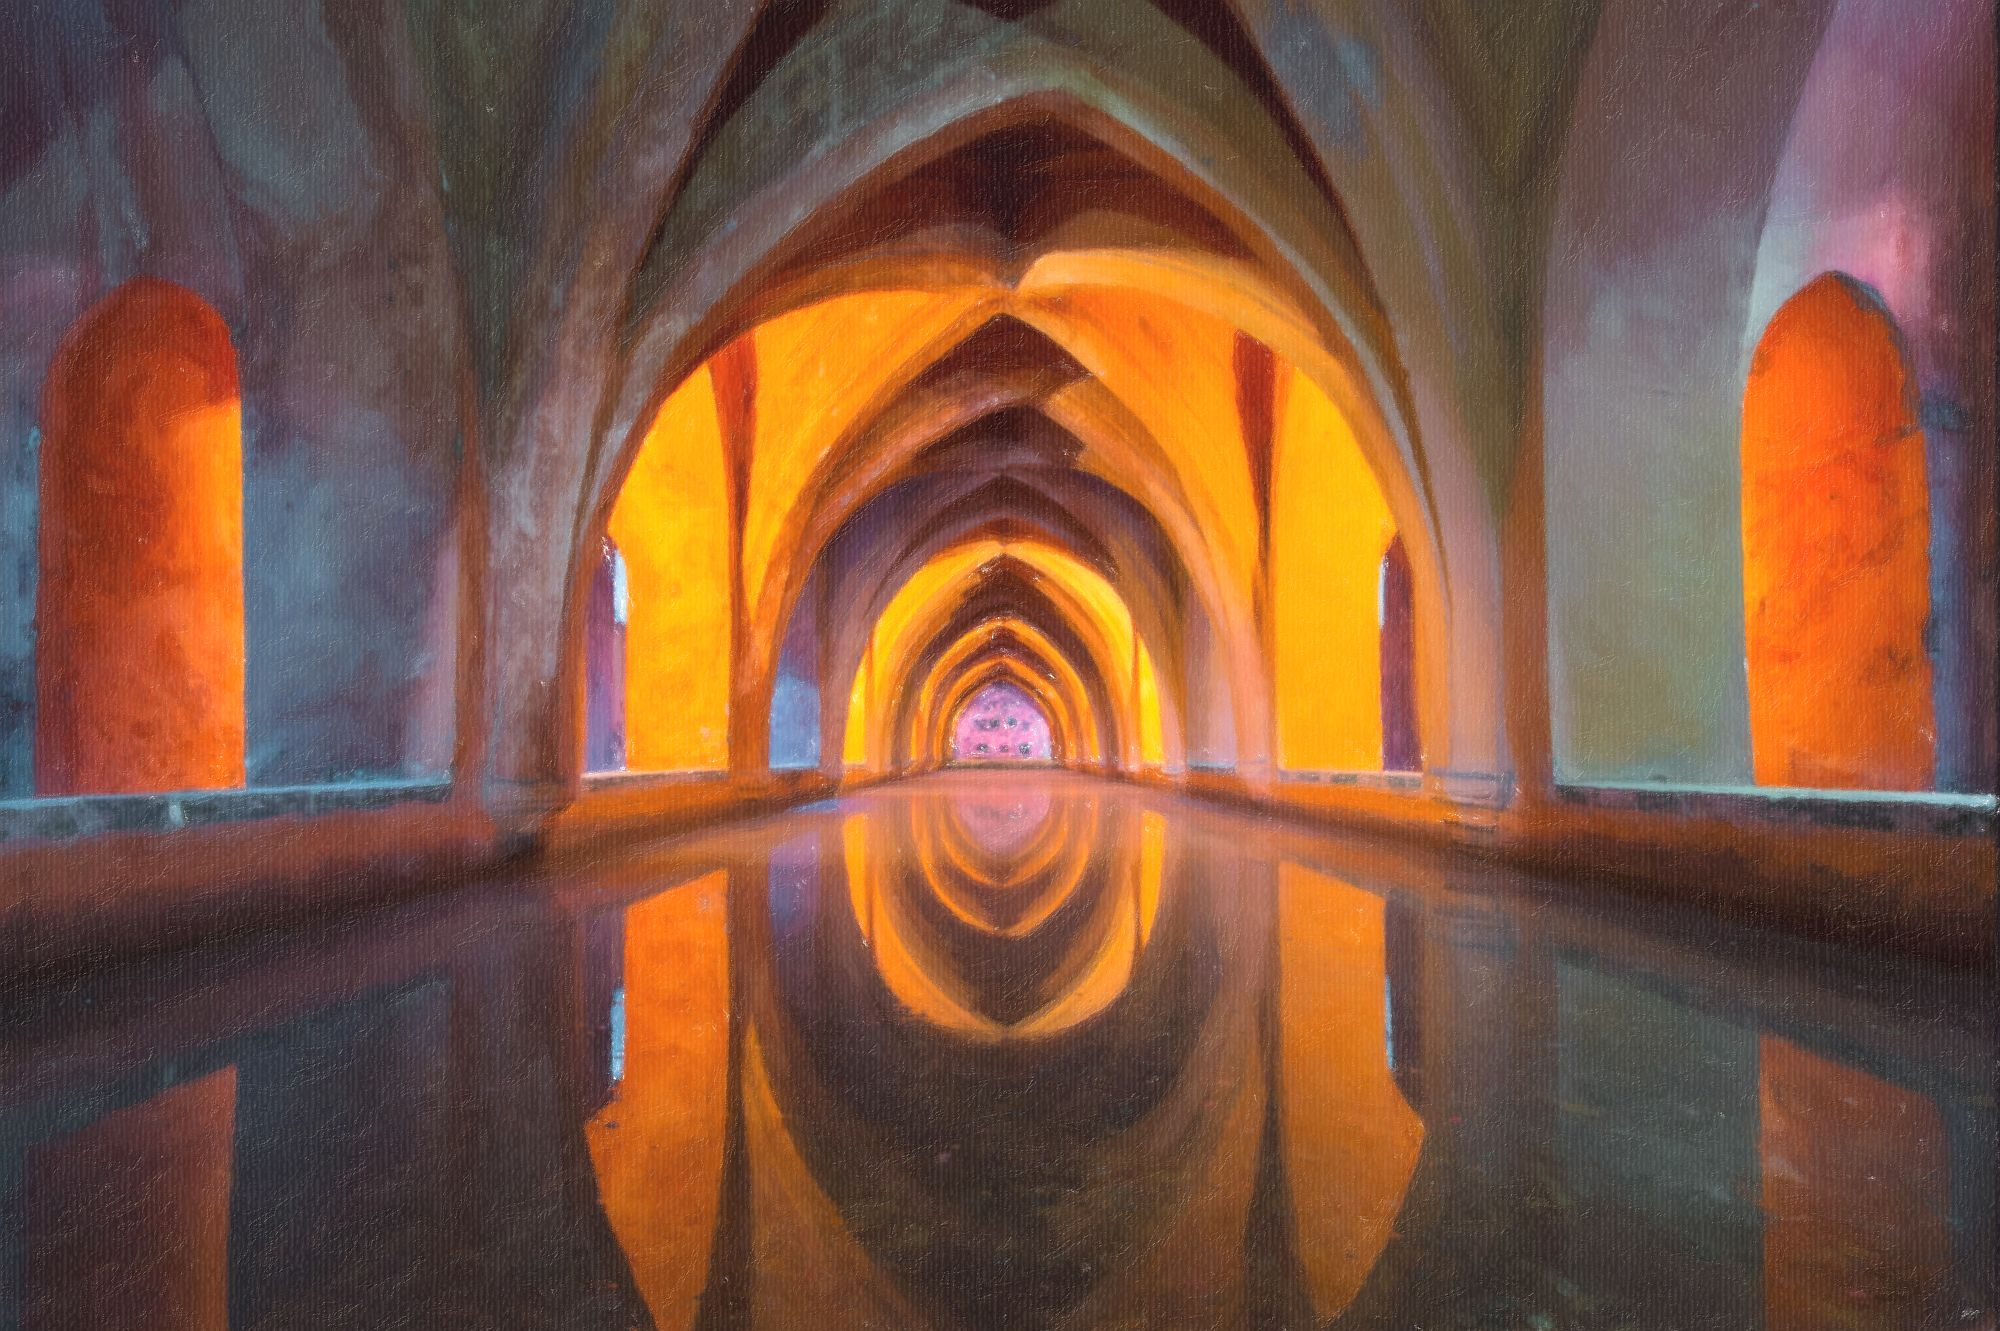
\includegraphics[width=\paperwidth,height=\paperheight]{cover.jpg}}}
}

% this is the small, square inset picture
\newcommand\BackgroundPicSmall{
 \put(0,0){\parbox[b][\textheight]{\textwidth}{%
 \vfill
 \centering
 \vspace{50em}
 {\setlength{\fboxsep}{5pt}%
  \fcolorbox{grey}{white}{%
 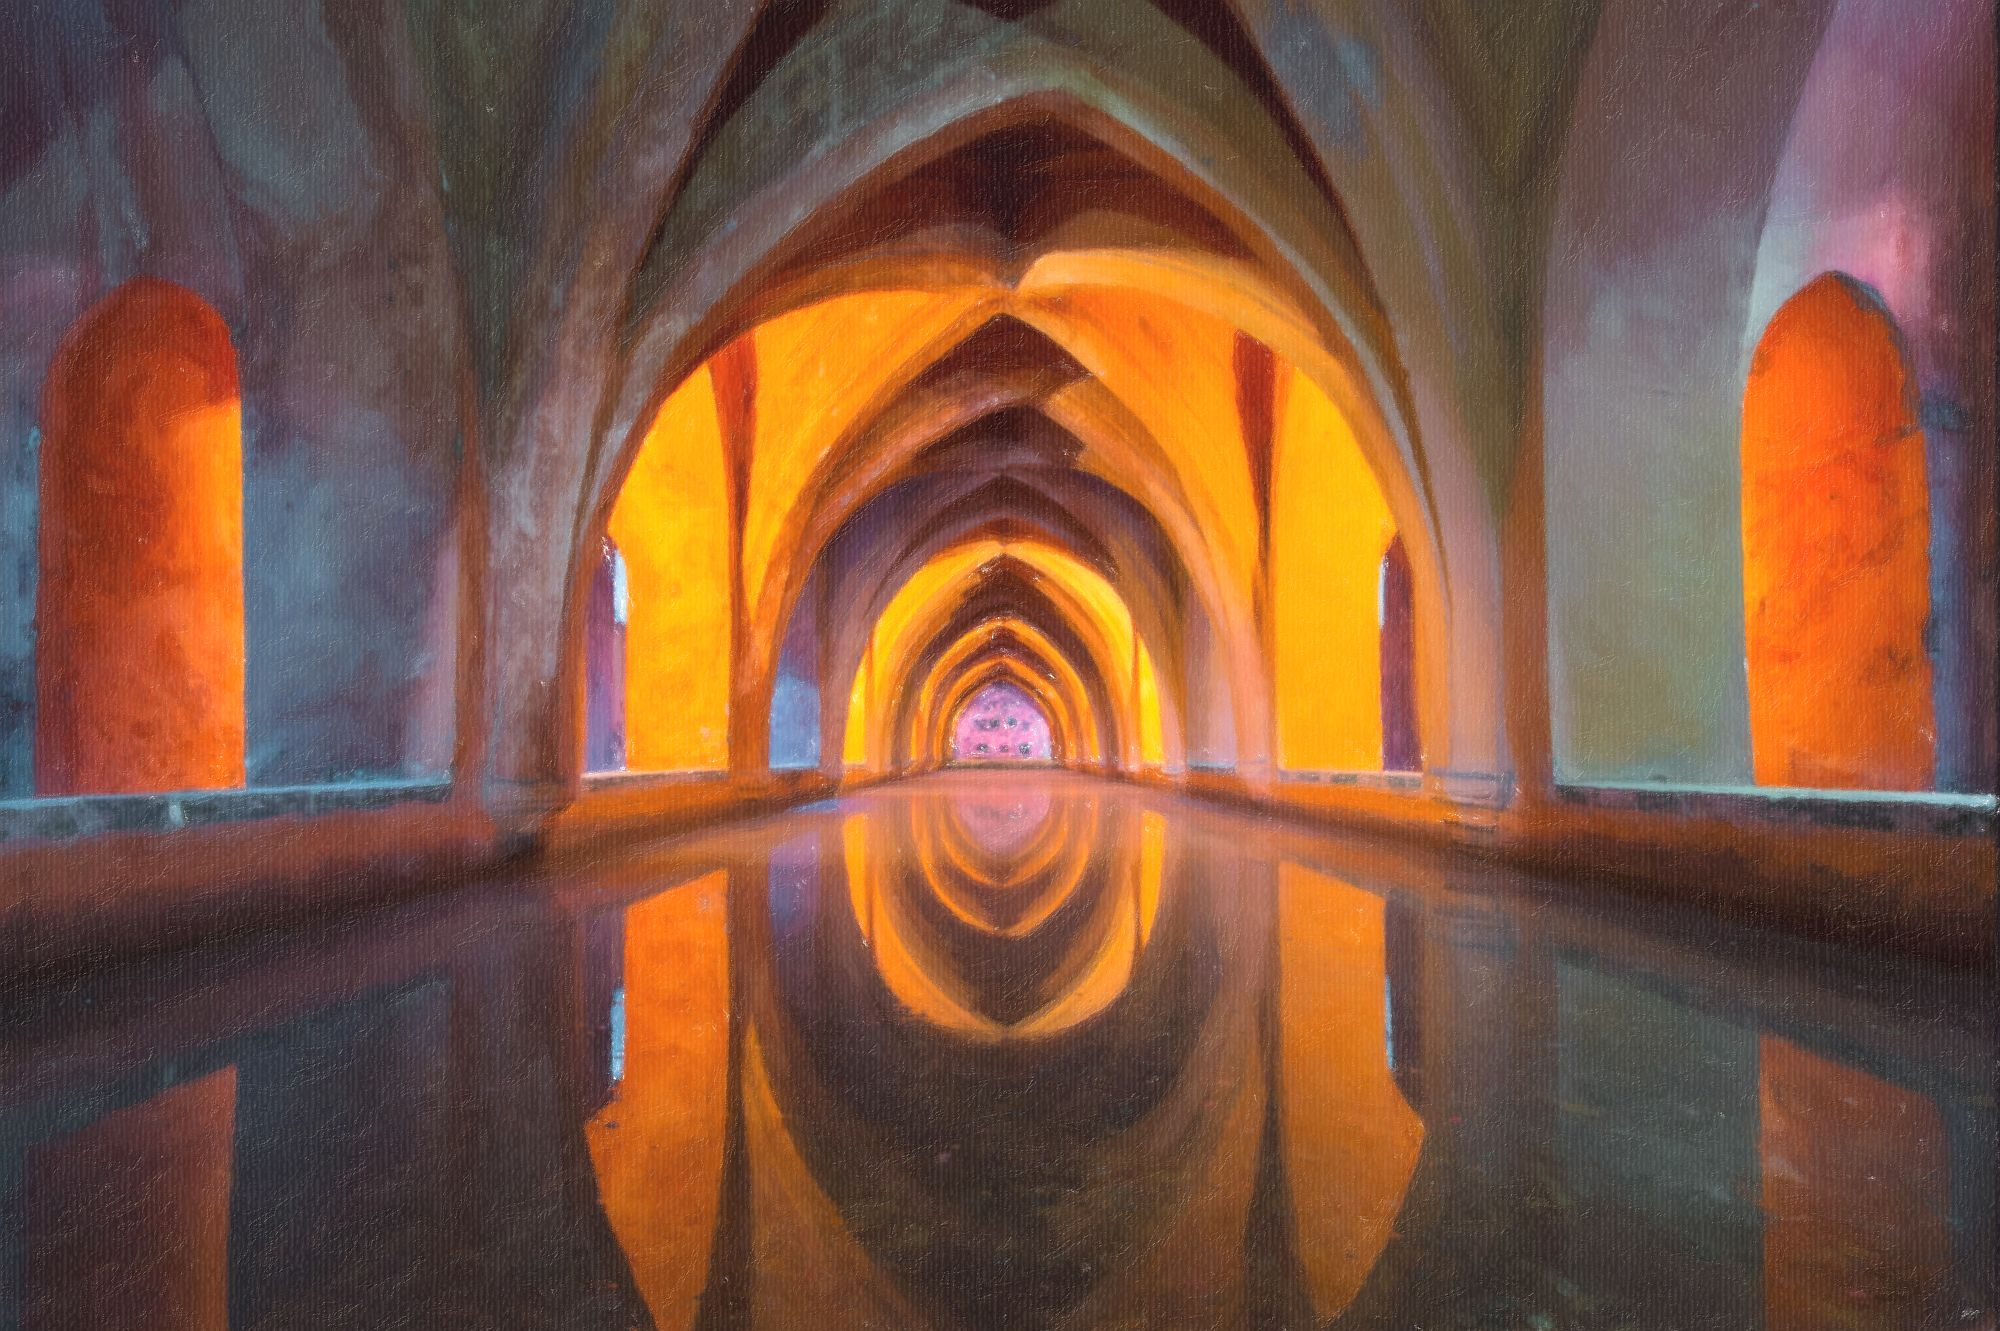
\includegraphics[width=\textwidth,height=0.65\textheight]{cover.jpg}}}%
 \vfill
 }}}

% this makes the table of contents linked to the rest of the PDF
\usepackage[hidelinks]{hyperref}
\hypersetup{
    colorlinks=false, %set true if you want colored links
    linktoc=all,     %set to all if you want both sections and subsections linked
}

\usepackage{paracol}

\makeatletter
